\Chapter{A szállítási probléma formalizálása}

\Section{A kiszállítási problémák általános modelljei}

Vizsgált esetek:

étterem: egy - több
futár: egy - több
kiszállítás: egy - több

(1, 1, 1)
(1, 1, *)
(*, 1, *)
(1, *, *)
(*, *, *)

\Section{Egy étterem, egy futár, egy kiszállítás esete.}

Ebben az esetben egy étterem található a városban, amelyből csak egy futár szállít ki mindig csak egy címre.
Bonyolultságát tekintve a legrövidebb utat kell megtalálni két pont között feltételezve azt, hogy egy pontból a másikba nem lehet közvetlenül eljutni, hanem más pontokat érintve csak. Ezáltal egy gráf élein kell végigmenni és közben keresni a legrövidebb a legrövidebb távot. Az optimális út meghatározása után venni kell ezen út hosszúnak kétszeresét, mivel a futár a szállítást követően vissza kell, hogy térjen az étterembe. Két pont közötti hossz meghatározására kiválló példa az egyik leginkább ismert algoritmus az A* algoritmus.

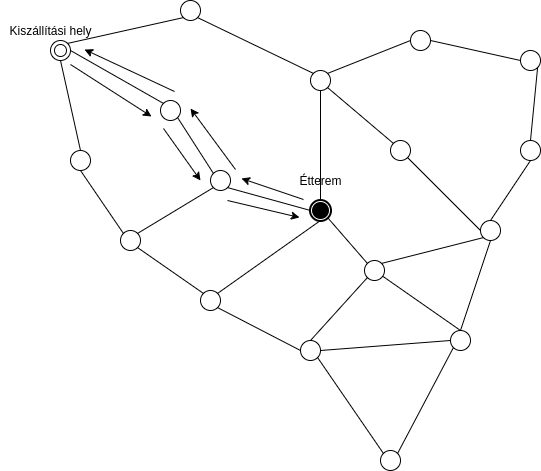
\includegraphics[scale=0.5]{images/Astar.png}

\Section{Egy étterem, egy futár, több kiszállítás esete.}

Egy étterem, egy futár és több kiszállításnál az adott helyzet egészen visszavezethető a klasszikus utazó ügynök problémához.
A futár elindul az étteremből, érinteni kell az összes kiszállítási pontot, valamint vissza kell érkeznie az étterembe, mindezt úgy, hogy a lehető legkisebb utat tegye meg.

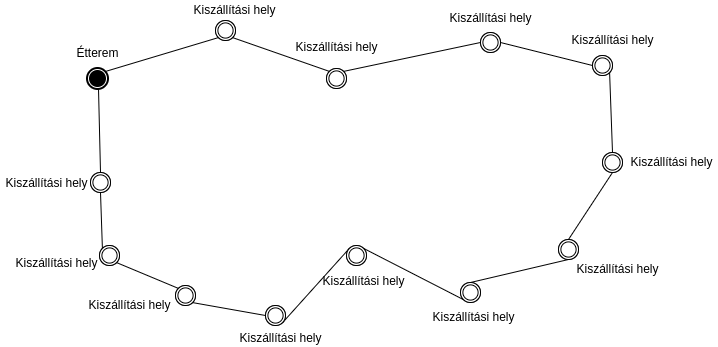
\includegraphics[scale=0.5]{images/Simpletsp.png}

\Section{Több étterem, egy futár, több kiszállítás esete}

Több étterem esetén meg kell határozni néhány feltételt. Jelen helyzetben a futár elindul az egyik étteremből kiszállít mindent, majd egy másik étterembe érkezik ezt követően és annak a rendeléseit is kiszállítja. Időben is meg kell szabni néhány határt, miszerint az első étteremből való indulás pillanatáig beérkezett rendeléseket szállítja csak ki az összes étteremből. Miután sikeresen kivitte az összes rendelést visszatér a kezdő étterembe és kezdődik előlről a folyamat. Maga a folyamat egy onmagát ismételő klasszikus utazó ügynök probléma, annyi eltéréssel, hogy nem ugyan abba az étterembe kell érkeznie ahonnan indult, hanem a hozzá legközelebb esőbe emibe még nem járt az adott ciklusban.

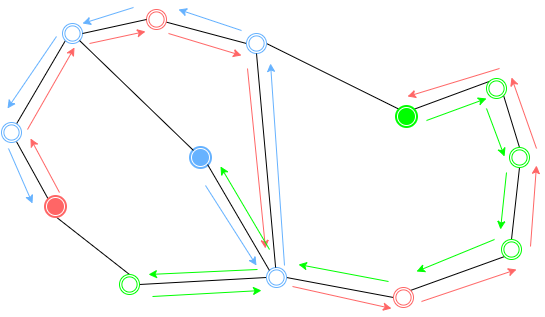
\includegraphics[scale=0.6]{images/Circulartsp.png}

\Section{Egy étterem, több futár, több kiszállítás esete}

Jelen eset reprezentálja az egy lerakatos több ügynökös utazó ügynök problémát. Feltételek meghatározásánál nélkülözhetetlen szempont, hogy határokat szabjunk az egyes futároknak, hogy ki milyen területre szállít ki. Ennek meghatározásánál fontos a kiszállítási címek közti táv figyelembe vétele. Ezek meghatározása után maga a probléma leegyszerűsíthető egy klasszikus utazó ügynök problémára.

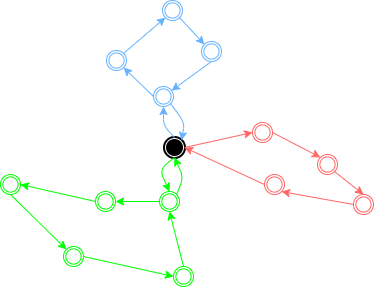
\includegraphics[scale=0.7]{images/Onedepotmtsp.png}

\Section{Több étterem, több futár, több kiszállítás esete}

Ez az eset tisztán leírja a több lerakatos több ügynökös utazó problémát. 